In this manuscript we discuss the problem of secure storage and transfer of access tokens between microservices.
Web browser may store access tokens both, in local storage or in cookie files.
Local storage is a web browser mechanism that allows web applications to store data locally on the user's device.
It is important to note that Local storage is vulnerable to Cross Site Scripting (XSS) attacks~\cite{spett2005cross}.
Cross Site Scripting (XSS) is a type of attack such that malicious JavaScript code is injected into an html-page
to access user's sensitive data, for example access tokens.
Cross Site Scripting (XSS) attacks may be divided by following groups:

\begin{itemize}
    \item \textbf{Reflected XSS} is a type of attack in which a malicious
    the script is passed to the web server via URL or form parameters and then returned back to the page's html code
    without proper filtering or escaping.\ If the user opens the page, then the script is executed
    in the browser, which can lead to the loss of sensitive data, such as access tokens.
    \item \textbf{Stored XSS} is a type of attack in which a malicious script is stored on the server, for example
    in the database and displayed on web pages.\ The script is executed in users' browsers,
    requesting pages with malicious code.
    \item \textbf{XSS in the DOM} is a type of attack such that a malicious script modifies the DOM tree of a web page,
    running in the user's browser.\ In most cases, based on modifying the URL string.
\end{itemize}

Another way to store credentials is to store them in cookie files.
Cookies are small pieces of data sent by web server and stored on user's device.
Storing access tokens in cookies eliminates potential XSS attacks since that HttpOnly setting
makes impossible to read cookies using JavaScript code.
Having credentials stored in cookies, HTTP request is performed via JavaScript.
If the object \texttt{\{ withCredentials: true \}} provided and auth cookies exist, then auth cookies are attached to request,
but cannot be accessed from JS code anyway.
Example of such request in TypeScript

\input{code_snippets/01_http_request_ts}

Note that cookie files are vulnerable to Cross-Site Request Forgery (CSRF) attacks~\cite{siddiqui2011cross}.
Cross-Site Request Forgery (CSRF) -- is an attack such that redirects user to the resource where user has active session.
It means that attacker could perform requests to resources on behalf of the user.
The main idea of Cross-Site Request Forgery (CSRF) attack is illustrated below

\begin{figure}[H]
    \centering
    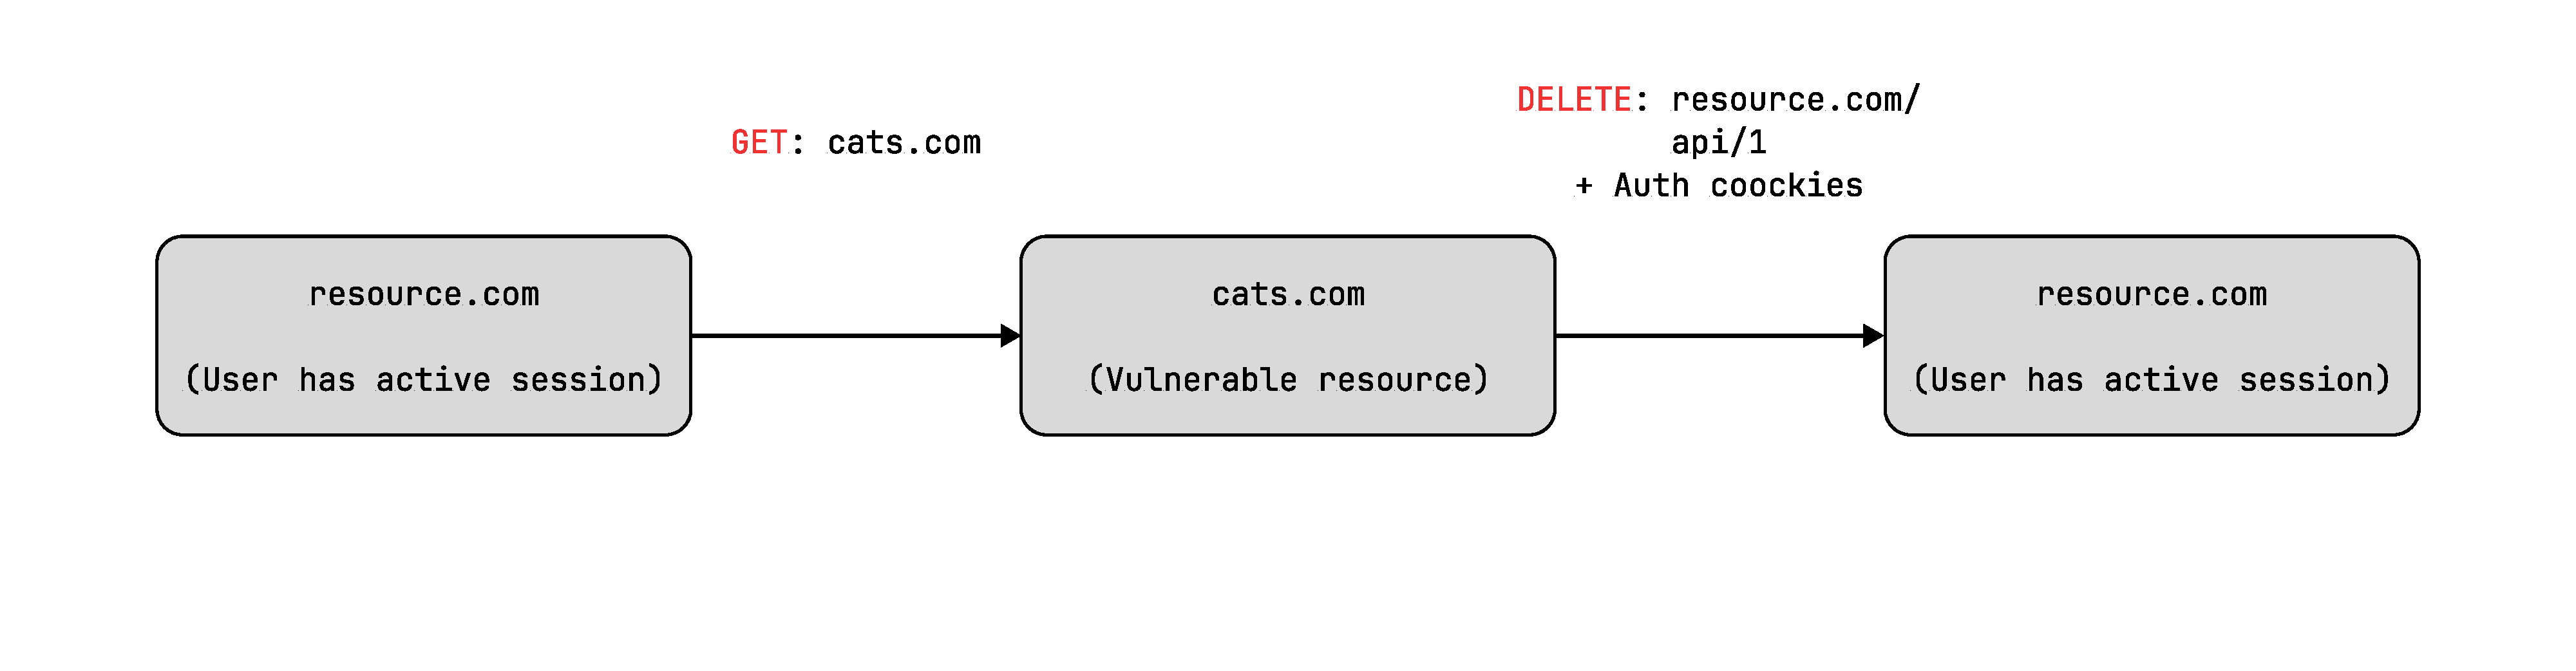
\includegraphics[width=1\textwidth]{img/Csrf_diagram}
    ~\caption{Cross-Site Request Forgery (CSRF) principle diagram.}\label{fig:csrf_diagram}
\end{figure}

Cookie files provided with \texttt{SameSite} setting that determines whether cookies will be sent
along with cross domain requests.

\texttt{SameSite} setting has one of the states below:

\begin{itemize}
    \item \textbf{None} -- means no restrictions are imposed on the transfer of cookies.
    \item \textbf{Lax} -- allows cookie transmission only by secure HTTP methods according to RFC 7231~\cite{fielding2014rfc}.
    These methods are \texttt{GET, HEAD, OPTIONS} and \texttt{TRACE}.
    \item \textbf{Strict} -- blocks cookies from being sent with any requests from third-party resources.
    Cookies will only be transferred within same domain.
\end{itemize}

Therefore, \texttt{SameSite} setting values such as \texttt{Lax} and \texttt{Strict} protect user from a CSRF attack
blocking submission of cookies using unsecure HTTP methods and cross domain requests.
There are more CSRF protection techniques in~\cite{owaspCsrf}.